% CHE374 Term Test 2 cheat sheet: double-sided, landscape A4 (PS5-8, Weeks 5-8).
% Compile from this folder: latexmk -pdf cheatsheet2.tex
\documentclass[8pt]{extarticle}
\usepackage[T1]{fontenc}
\usepackage[utf8]{inputenc}
\usepackage{lmodern}
\usepackage[a4paper,landscape,margin=0.45cm]{geometry}
\usepackage{amsmath,amssymb,mathtools}
\usepackage{multicol}
\usepackage{xcolor}
\usepackage{enumitem}
\usepackage{tikz}
\usetikzlibrary{decorations.pathreplacing}
\usepackage{array}
\usepackage{ragged2e}
\tikzset{every picture/.append style={scale=1.35,every node/.append style={transform shape}}}

\pagestyle{empty}
\setlength{\parindent}{0pt}
\setlength{\parskip}{0.6pt}
\setlength{\columnsep}{7pt}
\setlength{\columnseprule}{0.3pt}
\setlength{\fboxsep}{1.5pt}
\setlist{nosep,leftmargin=*,label=\textbullet,itemsep=0pt,topsep=0pt}
\setlength{\abovedisplayskip}{1pt}
\setlength{\belowdisplayskip}{1pt}
\setlength{\abovedisplayshortskip}{0pt}
\setlength{\belowdisplayshortskip}{0pt}
\setlength{\jot}{0.5pt}
\setlength{\tabcolsep}{2pt}
\renewcommand{\arraystretch}{1.0}
\thickmuskip=3mu plus 2mu
\medmuskip=2mu plus 1mu

\definecolor{navy}{RGB}{0,32,96}
\definecolor{dred}{RGB}{160,20,20}
\definecolor{dgreen}{RGB}{0,110,40}

% Section bar, red sub-heading, highlighted term, solving-logic box.
\newcommand{\sect}[1]{\par\vspace{1.5pt}\noindent\colorbox{navy}{\makebox[\dimexpr\linewidth-2\fboxsep][l]{\color{white}\bfseries\large #1}}\par\vspace{0.5pt}}
\newcommand{\sub}[1]{\par\noindent{\color{dred}\bfseries #1}\ }
\newcommand{\kw}[1]{{\color{dred}\bfseries #1}}
\newcommand{\logic}[2]{\par\vspace{1pt}\noindent\fcolorbox{orange!80!black}{yellow!12}{\parbox{\dimexpr\linewidth-2\fboxsep-2\fboxrule}{{\color{orange!50!black}\bfseries #1}\par #2}}\par\vspace{1pt}}
\newcommand{\ex}[1]{{\color{navy}\itshape #1}}
\newcommand{\bx}[1]{\fbox{$\displaystyle #1$}}
% Right-aligned bold answer at the end of a list line.
\newcommand{\ans}[1]{\unskip\nobreak\hfill\mbox{\textbf{#1}}}
% One-line worked application under an equation.
\newcommand{\use}[1]{\par{\color{navy}$\triangleright$\ \itshape #1}\par}

\begin{document}
\fontsize{9.0}{10.3}\selectfont
\begin{multicols*}{3}
\raggedcolumns
\RaggedRight

% =====================================================================
\sect{0. Test Pattern (2022--2024)}
\begin{enumerate}[label=\textbf{Q\arabic*},leftmargin=1.6em]
\item \kw{Compare alternatives}: periodic costs (resurfacing/overhaul every $k$ yr), finite life \& perpetuity, AW/PC, break-even benefit; or sequencing options in a max horizon.
\item \kw{IRR}: IRR of one project, incremental IRR (fill a blank), best project for several MARRs.
\item \kw{Depreciation}: $BV$ on Jan 1 of year $Y$ \& $D$ for year $Y$ by SL, DB, SOYD.
\item \kw{Statements}: cash plug, or T-accounts from transactions $\to$ IS + BS.
\end{enumerate}

% =====================================================================
\sect{1. Factors (MARR $=i$)}
\[\begin{array}{@{}ll@{}}
(F/P)=(1+i)^N & (P/F)=\dfrac{1}{(1+i)^N}\\[6pt]
(P/A)=\dfrac{(1+i)^N-1}{i(1+i)^N} & (A/P)=\dfrac{i(1+i)^N}{(1+i)^N-1}\\[6pt]
(F/A)=\dfrac{(1+i)^N-1}{i} & (A/F)=\dfrac{i}{(1+i)^N-1}
\end{array}\]
\[\text{Perpetuity: }\bx{P=\frac Ai}\ (\text{1 period before 1st }A)\]
\[(P/\text{Geom},i,g,N)=\frac{1-\left(\frac{1+g}{1+i}\right)^N}{i-g}\]
\sub{Interpolate:} $\bx{x\approx x_1+(x_2-x_1)\dfrac{y^*-y_1}{y_2-y_1}}$ \ (bracket the target tightly; answer must lie between $x_1,x_2$).

% =====================================================================
\sect{2. PW / AW / Comparing Projects}
\begin{itemize}
\item \kw{Independent}: accept each with PW $>0$. \kw{Mut.\ exclusive}: best PW/AW (or lowest PC/AC). \kw{Budget}: list feasible combos, pick best.
\item Costs only: $PC=-PW$, $AC=-AW$; pick \kw{lowest}.
\end{itemize}
\[\bx{AW=PW\,(A/P,i,N)}\]
\[AW=-FC(A/P,i,N)+\text{net annual}+S(A/F,i,N)\]
\begin{itemize}
\item Different lives: PW over \kw{LCM}, or AW of \kw{one life} (repeated identical lives have the same AW).
\item Fixed horizon $\to$ \kw{study period}: build actual plans; unused life lost (or use given salvage).
\item Same life: PW and AW give the same ranking.
\end{itemize}

% =====================================================================
\sect{3. Periodic Costs (every $k$ yrs)}
\[\bx{i_k=(1+i)^k-1}\quad\text{(effective rate per $k$-yr period)}\]
\sub{Finite life $N$:} count occurrences $k,2k,\dots<N$ ($n=\lfloor N/k\rfloor$, none at retirement):
\[PW=X\,(P/A,i_k,n)=X\sum_{j=1}^{n}\frac{1}{(1+i)^{jk}}\]
\sub{Perpetuity} (first cost once):
\[\bx{PC=FC+\frac{\text{O\&M}}{i}+\frac{X}{i_k}}\]
\[\bx{AC=FC\cdot i+\text{O\&M}+\frac{X}{i_k}\,i}\quad\Big(\tfrac{X}{i_k}i=X(A/F,i,k)\Big)\]
If FC repeats every $L$ yrs: use $FC(A/P,i,L)$ instead of $FC\cdot i$.
\[\text{Component AC: }\text{O\&M}+\big[FC+X(P/A,i_k,n)\big](A/P,i,N)\]
\sub{Break-even benefit $B$} (B gives extra benefit/yr): set $PC_A=PC_B-B(P/A,i,N)$:
\[\bx{B=\frac{PC_B-PC_A}{(P/A,i,N)}}\qquad\text{perpetuity: }B=(PC_B-PC_A)\,i\]
\use{2022: $5.7$M every 6 yr at 5\%: $i_6=0.3401$; $PC_A=38\text{M}+380\text{k}(P/A,5\%,50)+5.7\text{M}(P/A,0.3401,8)$.}

% =====================================================================
\sect{4. Sequencing Options (max horizon)}
Revenue at end of each cycle of length $n$:
\[AW=\text{Rev}(A/F,i,n)-\text{O\&M}-FC(A/P,i,n)\]
\[\bx{PW_{1\to2}=AW_1(P/A,i,n_1)+AW_2(P/A,i,n_2)(P/F,i,n_1)}\]
\begin{itemize}
\item List plans with total length $\le$ horizon; compare PW.
\item Same pair, either order: put the \kw{higher-AW} option first.
\item Replacement used only briefly $\to$ low first cost wins (PS5 Q4: B then A).
\end{itemize}

% =====================================================================
\sect{5. Loans \& Growing Deposits}
\[A=P(A/P,i,N),\quad \text{Int}_k=i\,B_{k-1},\quad \text{Prin}_k=A-\text{Int}_k\]
\[B_k=A(P/A,i,N-k)=P(F/P,i,k)-A(F/A,i,k)\]
\[\text{Principal share of payment }k=\frac{1}{(1+i)^{N-k+1}}\]
\sub{\% of salary $X$:} $X S_1(P/\text{Geom},i,g,N)=F(P/F,i,N)$. Quarterly deposits $\to$ year-end factor $\tfrac14\sum_{q}(1+i)^{q/4}$, $q=0..3$.

% =====================================================================
\sect{6. IRR}
\[\bx{0=-FC+A(P/A,i^*,N)+S(P/F,i^*,N)}\]
\begin{itemize}
\item No salvage: $(P/A,i^*,N)=FC/A$ $\to$ tables, interpolate.
\item Two cash flows: $i^*=(F/P)^{1/N}-1$.
\item \kw{Simple} investment ($-$ then $+$): one IRR; accept if $\bx{IRR>MARR\iff PW(MARR)>0}$.
\item Sign changes $>1$: may have multiple IRRs $\to$ use PW.
\end{itemize}
\sub{Quick check vs MARR:} plug $i=$MARR into the PW; $PW>0\Rightarrow IRR>$MARR (no exact IRR needed).
\begin{center}
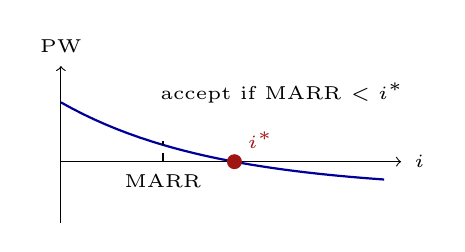
\begin{tikzpicture}[x=0.32cm,y=0.18cm,font=\tiny]
\draw[->](0,0)--(10,0)node[right]{$i$}; \draw[->](0,-3.2)--(0,5)node[above]{PW};
\draw[thick,blue!60!black,domain=0:9.5,samples=30] plot(\x,{4.6*exp(-0.22*\x)-1.5});
\fill[dred](5.1,0)circle(2pt)node[above right]{$i^*$};
\draw[dashed](3,0)node[below]{MARR}--(3,1.06);
\node at (6.5,3.6){accept if MARR $<i^*$};
\end{tikzpicture}
\end{center}

% =====================================================================
\sect{7. Incremental IRR (mut.\ exclusive)}
Higher IRR $\neq$ better (scale ignored). Compare the \kw{increment}.
\begin{enumerate}[leftmargin=1.3em,label=\arabic*.]
\item Order by first cost. Current best $=$ \kw{Null}.
\item Challenger vs current best: entry (row challenger, \kw{column current best}) $=IRR_{X-Y}$.
\item $IRR_\Delta>$MARR $\Rightarrow$ challenger becomes best; else keep.
\item Repeat to the last project. $=$MARR: \kw{tie}.
\end{enumerate}
\[\text{Increment }X-Y:\ 0=-\Delta FC+\Delta A(P/A,r,N)+\Delta S(P/F,r,N)\]
\begin{itemize}
\item Projects with own IRR $<$ MARR can be dropped first.
\item $\Delta$ can be negative (e.g.\ $-10.96\%$): still compare to MARR.
\item ``Highest PW at MARR $m$'' $=$ run the procedure at $m$.
\item Check: $PW_X-PW_Y=PW_{X-Y}$.
\end{itemize}
\sub{Budget (de facto MARR):} rank independent projects by IRR, fund down the list until the budget runs out; cutoff $=$ IRR of last funded.
\sub{Payback} $=FC/\text{annual savings}$ (ignores TVM \& later flows).

% =====================================================================
\sect{8. Depreciation}
$B$ basis, $S$ salvage, $N$ life, $BV_0=B$, $BV_t=B-\sum_{j\le t}D_j$.
\[\text{SL: }\bx{D=\frac{B-S}{N}},\quad BV_t=B-tD\]
\[\text{DB: }\bx{D_t=d\,BV_{t-1}},\quad BV_t=B(1-d)^t\]
\[\bx{d=1-\Big(\frac SB\Big)^{1/N}}\quad\text{DDB: }d=\frac2N\]
Fixed $d$ given: use it ($BV_N\neq S$ in general).
\[\text{SOYD}_N=\frac{N(N+1)}2,\quad\bx{D_t=\frac{N-t+1}{\text{SOYD}_N}(B-S)}\]
\[\bx{BV_t=B-\frac{\text{SOYD}_N-\text{SOYD}_{N-t}}{\text{SOYD}_N}(B-S)}\]
\[\text{Units of prod.: }D_t=\frac{\text{units}_t}{\text{lifetime units}}(B-S)\]
\sub{Dates $\to$ index:} bought Jan 1 of year $Y_0$. Jan 1 of $Y$ $=$ end of year $t=Y-Y_0$ $\Rightarrow BV_t$; depreciation \emph{for} year $Y$ $=D_{t+1}$.
\begin{center}
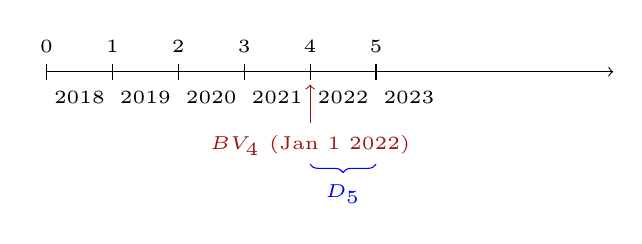
\begin{tikzpicture}[x=0.62cm,y=0.3cm,font=\tiny]
\draw[->](0,0)--(8.6,0);
\foreach \x/\y in {0/2018,1/2019,2/2020,3/2021,4/2022,5/2023}{\draw(\x,.25)--(\x,-.25);\node[above] at (\x,0.2){\x};\node[below] at (\x+0.5,-0.2){\y};}
\draw[->,dred](4,-1.6)node[below]{$BV_4$ (Jan 1 2022)}--(4,-0.4);
\draw[decorate,decoration={brace,mirror,amplitude=3pt},blue](4,-2.9)--(5,-2.9)node[midway,below=2pt]{$D_5$};
\end{tikzpicture}
\end{center}
\use{2022 test: $B=450$k, $S=50$k, $N=8$, Jan 1 2018 $\to$ Jan 1 2022: SL $BV_4=250$k, $D=50$k; DB $d=0.2402$, $BV_4=150$k, $D_5=36.0$k; SOYD$=36$, $BV_4=450-\tfrac{26}{36}400=161.1$k, $D_5=\tfrac4{36}400=44.4$k.}
\sub{Sold at MV vs book value $BV$:}
\begin{itemize}
\item $MV<BV$: \kw{loss on disposal} $BV-MV$ (extra $D$).
\item $BV<MV\le B$: \kw{recaptured dep.} $MV-BV$ (negative $D$).
\item $MV>B$: \kw{capital gain} $MV-B$ $+$ recapture $B-BV$.
\end{itemize}
Life re-evaluated: depreciate current $BV$ over the new remaining life.

% =====================================================================
\sect{9. Accounting Basics}
\[\bx{\text{Assets}=\text{Liabilities}+\text{Equity}}\]
Balance sheet $=$ snapshot; income statement $=$ over a period. Accrual: record when it \kw{happens}, not when cash moves.
\begin{center}
\begin{tabular}{|l|c|c|}\hline
Account & Debit & Credit\\\hline
Assets, Expenses, Dividends & $+$ & $-$\\
Liabilities, Equity, Revenue & $-$ & $+$\\\hline
\end{tabular}
\end{center}
Every entry: total Dr $=$ total Cr. Expenses are debits because they \kw{reduce equity}.
\[\bx{RE_{\text{end}}=RE_{\text{begin}}+NI-\text{Div}}\]
$NI-\text{Div}=$ addition to equity. Dividend payout ratio $q$: Div $=q\,NI$.

% =====================================================================
\sect{10. Transactions $\to$ Entries}
\begin{center}
\renewcommand{\arraystretch}{1.05}
\begin{tabular}{|p{0.43\linewidth}|p{0.24\linewidth}|p{0.24\linewidth}|}\hline
\textbf{Transaction} & \textbf{Dr} & \textbf{Cr}\\\hline
Owner/partner invests & Cash & Paid-in cap.\\
Borrow from bank & Cash & Debt\\
Buy inventory on account (payables) & Inventory & A/P\\
Sale for cash & Cash & Revenue\\
Sale on account / ``non-cash revenue'' & A/R & Revenue\\
Inventory sold / audit says COGS $=x$ & COGS & Inventory\\
Paid \kw{manufacturing} wages \& utilities & COGS & Cash\\
Paid salaries, selling \& admin & SG\&A & Cash\\
Collect receivables & Cash & A/R\\
Pay payables & A/P & Cash\\
Depreciation & Dep.\ exp. & PP\&E net\\
Interest paid / accrued & Int.\ exp. & Cash / Int.\ pay.\\
Taxes incurred, not paid & Tax exp. & Taxes pay.\\
Pay taxes owed & Taxes pay. & Cash\\
Pay dividend & Dividends & Cash\\
Prepay next month's rent & Prepaid & Cash\\
Buy stocks (short term) & Investments & Cash\\
Buy land / equipment & Land / PP\&E & Cash\\\hline
\end{tabular}
\end{center}
\kw{Not} income-statement items: collecting A/R, paying A/P, dividends, prepaying, buying assets, owner investment, borrowing.

% =====================================================================
\sect{11. T-Account Procedure}
\begin{enumerate}[leftmargin=1.3em,label=\arabic*.]
\item Post each transaction (number it) to two accounts.
\item Net each account $=$ change for the period.
\item IS from revenue/expense accounts.
\item BS: \kw{closing $=$ opening $+$ change}; RE via formula.
\item Check A $=$ L $+$ E.
\end{enumerate}
\begin{center}
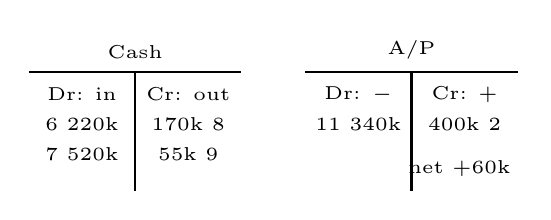
\begin{tikzpicture}[x=0.5cm,y=0.35cm,font=\tiny]
\draw[thick](0,0)--(4,0);\draw[thick](2,0)--(2,-3.2);\node[above] at (2,0){Cash};
\node at (1,-0.6){Dr: in};\node at (3,-0.6){Cr: out};
\node at (1,-1.4){6\ 220k};\node at (3,-1.4){170k\ 8};
\node at (1,-2.2){7\ 520k};\node at (3,-2.2){55k\ 9};
\begin{scope}[xshift=2.6cm]
\draw[thick](0,0)--(4,0);\draw[thick](2,0)--(2,-3.2);\node[above] at (2,0){A/P};
\node at (1,-0.6){Dr: $-$};\node at (3,-0.6){Cr: $+$};
\node at (1,-1.4){11\ 340k};\node at (3,-1.4){400k\ 2};
\node at (2.9,-2.6){net $+60$k};
\end{scope}
\end{tikzpicture}
\end{center}

% =====================================================================
\sect{12. Income Statement}
\begin{center}
\begin{tabular}{@{}ll@{}}
Revenue & \\
$-$ COGS (materials, mfg labour) & $=$ \textbf{Gross margin}\\
$-$ SG\&A, indirect, misc.\ & $=$ \textbf{EBITDA}\\
$-$ Depreciation & $=$ \textbf{EBIT}\\
$-$ Interest, $\pm$ other loss (gain) & $=$ \textbf{EBT}\\
$-$ Taxes ($t\times$EBT) & $=$ \textbf{Net income}\\
$-$ Dividends & $=$ \textbf{Addition to equity}
\end{tabular}
\end{center}
Expenses written as positive numbers; a gain in a ``loss (gain)'' line is negative.

% =====================================================================
\sect{13. Balance Sheet \& Cash Plug}
\begin{itemize}
\item \kw{Current assets}: cash, A/R, inventory, prepaid, short-term investments.
\item \kw{Noncurrent}: land, PP\&E net, other long-term assets.
\item \kw{Current liab.}: A/P, wages pay., taxes pay., interest pay., short-term debt.
\item \kw{Noncurrent liab.}: bank loan (due in years), bonds, other \emph{long-term} liab.
\item \kw{Equity}: common stock / paid-in capital, retained earnings.
\end{itemize}
\sub{Cash plug:} IS $\to NI$ $\to RE_{\text{end}}$ $\to$ total L $+$ E $\to$
\[\bx{\text{Cash}=(L+E)-\text{(all other assets)}}\]
Taxes ``all paid'' $\Rightarrow$ no taxes payable. Use \emph{beginning} RE given.
\use{2022: Sales 4950, COGS 2560, SG\&A 490, Dep 160, Int 400, tax 20\%: NI $=1072$, Div (50\%) $=536$, RE $=2450+536=2986$.}

% =====================================================================
\sect{14. Ratios}
\[\text{Current ratio}=\frac{\text{current assets}}{\text{current liabilities}}\]
\[\text{Quick ratio}=\frac{\begin{array}{@{}c@{}}\text{cash}+\text{short-term investments}\\+\ \text{accounts receivable}\end{array}}{\text{current liabilities}}\]
\[\text{Inventory turnover}=\frac{\text{cost of goods sold}}{\text{average inventory}}\]
\[\text{Days of inventory}=\frac{365}{\text{inventory turnover}}\]
\[\text{A/R turnover}=\frac{\text{sales}}{\text{average accounts receivable}}\]
\[\text{Days of A/R}=\frac{\text{average accounts receivable}}{\text{sales}/365}\]
\[\text{Debt ratio}=\frac{\text{total liabilities}}{\text{total assets}}\]
\[\text{Equity ratio}=\frac{\text{total equity}}{\text{total assets}}=1-\text{debt ratio}\]
\[\text{Debt-to-equity}=\frac{\text{total liabilities}}{\text{total equity}}\ \text{(or debt only)}\]
\[\text{Times interest earned}=\frac{\text{EBIT}}{\text{interest expense}}\]
\[\text{Profit margin}=\frac{\text{net income}}{\text{sales}}\qquad\text{ROA}=\frac{\text{net income}}{\text{total assets}}\]
\[\bx{\text{ROE}=\frac{\text{net income}}{\text{total equity}}}\]
\[\text{EPS}=\frac{\text{net income}}{\text{shares outstanding}}\qquad\text{P/E}=\frac{\text{share price}}{\text{EPS}}\]
\[\text{Dividend yield}=\frac{\text{dividends per share}}{\text{share price}}\]
Monthly IS: annualize $\times\frac{365}{30}$ (or $\times12$); state the period. More leverage $\Rightarrow$ riskier, higher \emph{expected} ROE.

% =====================================================================
\sect{15. Traps}
\begin{itemize}
\item Dividends are not an expense; prepaid rent is an asset.
\item Collecting A/R / paying A/P: no revenue/expense.
\item Mfg wages $\to$ COGS; office/selling $\to$ SG\&A.
\item Gain on investments goes after EBIT.
\item Incremental IRR: use the \kw{current best}'s column.
\item $A/i$ sits 1 period before the first payment.
\item Periodic costs: no occurrence at end of life.
\item DB $D_{t+1}=d\,BV_t$, not $d\,B$.
\item Round only at the end (keep $d$, $i_k$ to 4+ decimals).
\end{itemize}

% =====================================================================
\sect{16. Interpreting Ratios (written part)}
\begin{itemize}
\item \kw{Current / quick} higher: easier to pay short-term bills, less risk.
\item \kw{Inventory turnover} higher: sells stock faster, more efficient.
\item \kw{A/R days} lower: collects from customers faster.
\item \kw{A/P days} higher: holds cash longer (free supplier credit); lower $=$ pays faster, less cash on hand.
\item \kw{Equity ratio} lower ($=$ more debt): riskier for shareholders, so they expect a \emph{higher} return; $\text{ROE}=\text{ROA}\times\frac{\text{total assets}}{\text{total equity}}$.
\item \kw{TIE} higher: covers interest more easily.
\end{itemize}

% =====================================================================
\sect{17. Past-Test Answers (check method)}
\begin{itemize}
\item \textbf{2024 Q1} (5\%, $\infty$ life): $i_{15}=1.0789$, $i_9=0.5513$; $AC_A=500\text{k}(.05)+10\text{k}+\frac{330\text{k}}{1.0789}(.05)=50{,}293$; $AC_B=66{,}173$ $\Rightarrow$ A.
\item \textbf{2023 Q1} (10\%, max 6 yr): $AW_{DF}=7{,}035$, $AW_{NF}=8{,}242$, $AW_{SP}=6{,}500$; $PW_{DF\to SP}=7035(P/A,4)+6500(P/A,2)(P/F,4)=30{,}806<PW_{NF}=31{,}243$ $\Rightarrow$ NF.
\item \textbf{2023 Q2} (12\%): only B, D beat MARR; $D-B$: $-66\text{k}+14\text{k}(P/A,r,8)+5\text{k}(P/F,r,8)$, $PW(12\%)=+0.6\text{k}$ ($r=12.25\%$) $\Rightarrow$ D.
\item \textbf{2024 Q2}: $D-B$: $0=-140+37(P/A,r,5)\Rightarrow r=10.07\%$.
\item \textbf{2023 Q3}: $B=750$k, $S=50$k, $N=12$, Jan 1 2015 $\to$ 2021 ($t=6$): SL $BV_6=400$k, $D_7=58.3$k; DB $d=.2020$, $BV_6=193.6$k, $D_7=39.1$k; SOYD$=78$, $BV_6=750-\frac{78-21}{78}700=238.5$k, $D_7=\frac6{78}700=53.8$k.
\item \textbf{2024 Q3}: COGS $=440\text{k}$ (audit) $+170\text{k}$ (mfg wages) $=610\text{k}$; NI $=36$k.
\end{itemize}

\end{multicols*}
\end{document}
